\documentclass[12pt]{article}
\usepackage{tikz}

\begin{document}

\begin{center}
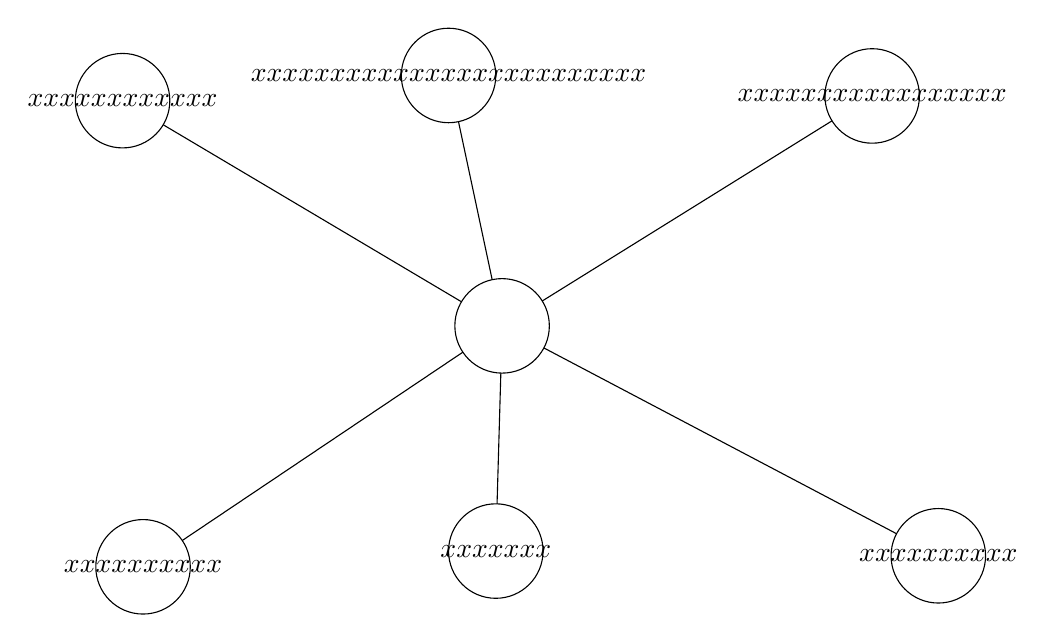
\begin{tikzpicture}[scale=0.2]
\tikzstyle{every node}+=[inner sep=0pt]
\draw [black] (13.1,-14.9) circle (3);
\draw (13.1,-14.9) node {$xxxxxxxxxxxx$};
\draw [black] (33.8,-13.3) circle (3);
\draw (33.8,-13.3) node {$xxxxxxxxxxxxxxxxxxxxxxxxx$};
\draw [black] (60.7,-14.6) circle (3);
\draw (60.7,-14.6) node {$xxxxxxxxxxxxxxxxx$};
\draw [black] (37.2,-29.2) circle (3);
\draw [black] (14.4,-44.5) circle (3);
\draw (14.4,-44.5) node {$xxxxxxxxxx$};
\draw [black] (36.8,-43.5) circle (3);
\draw (36.8,-43.5) node {$xxxxxxx$};
\draw [black] (64.9,-43.8) circle (3);
\draw (64.9,-43.8) node {$xxxxxxxxxx$};
\draw [black] (16.89,-42.83) -- (34.71,-30.87);
\draw [black] (36.88,-40.5) -- (37.12,-32.2);
\draw [black] (39.85,-30.6) -- (62.25,-42.4);
\draw [black] (39.75,-27.62) -- (58.15,-16.18);
\draw [black] (36.57,-26.27) -- (34.43,-16.23);
\draw [black] (15.68,-16.43) -- (34.62,-27.67);
\end{tikzpicture}
\end{center}

\end{document}
